\section{Appendix}\label{sec:appendix}

% Appendices do not count toward the page limit.
\begin{figure}[h]
    \centering
    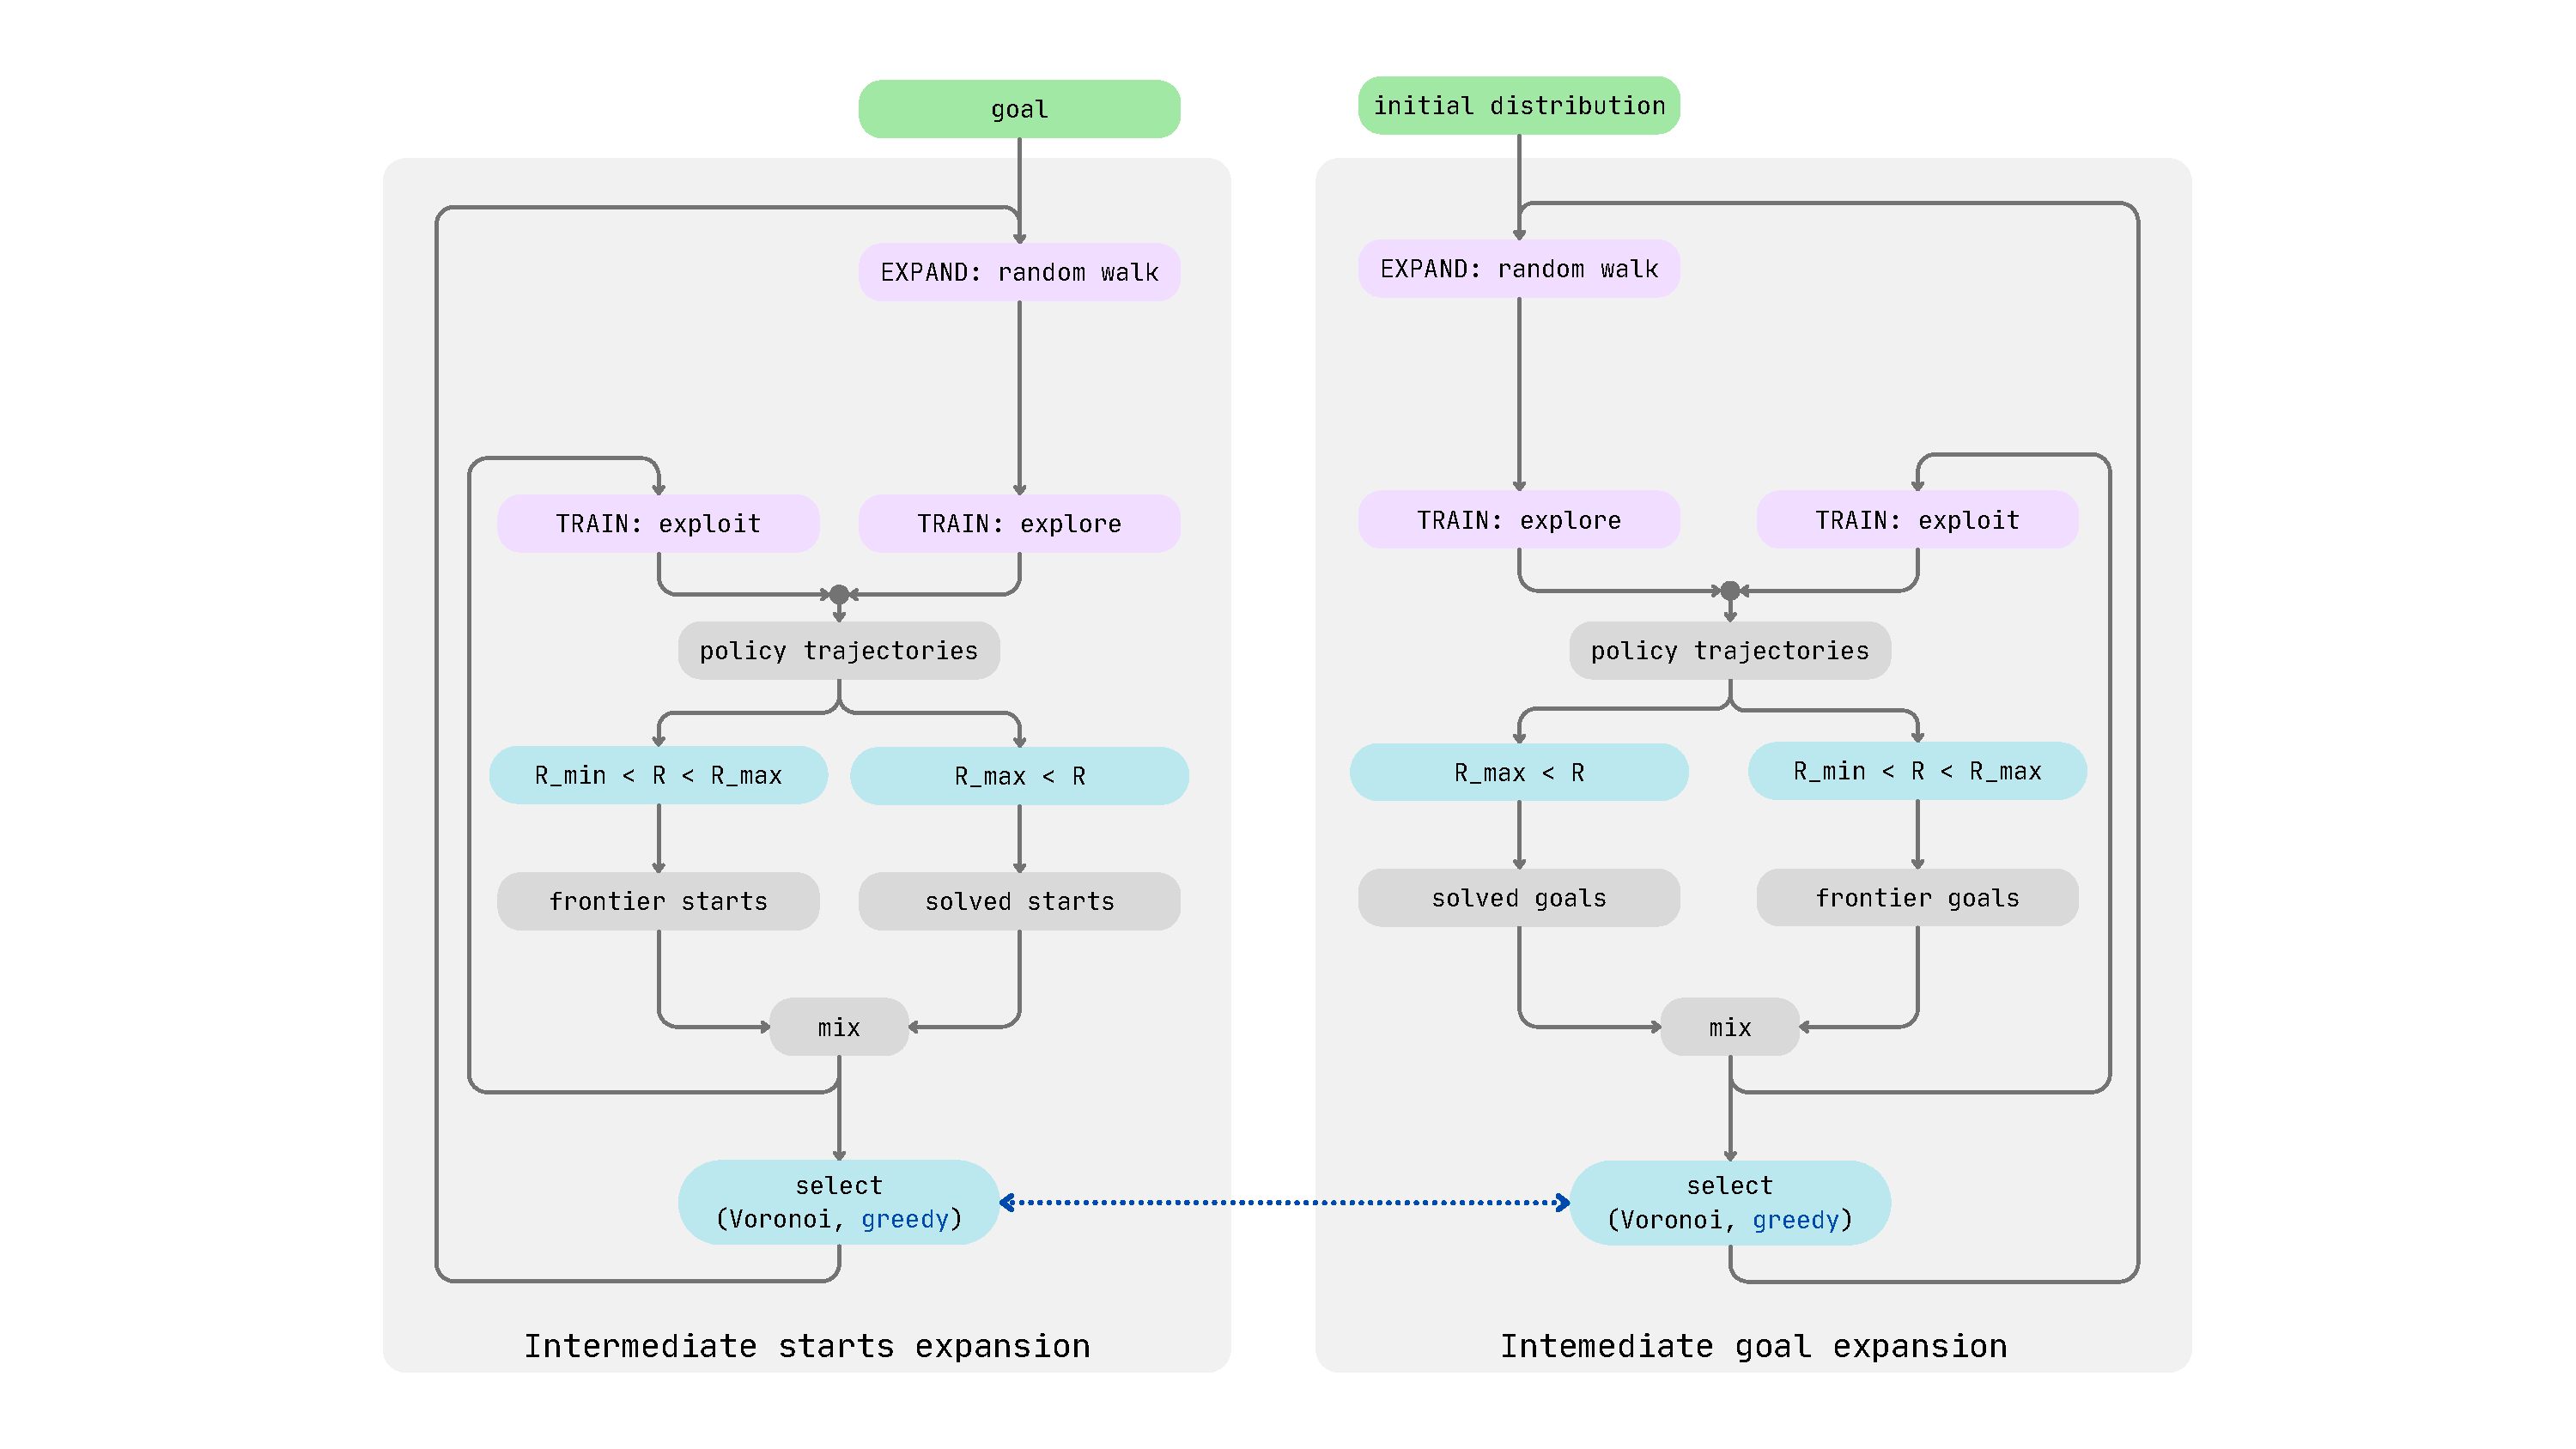
\includegraphics[width=\linewidth]{img/graphics/scheme_full.pdf}
    \caption{Overview of BVER. Both expansions run the same loop: random walks seeded in the goal (left) or the initial distribution (right) propose new starts or goals (explore), which are trained on together with the mixed training set (exploit). Rollout returns $R$ split the trained states into frontier ($R_{\min} < R < R_{\max}$) and solved ($R_{\max} \leq R$) states, which are mixed into the next training set. The seeds of the next random walks are selected from this set by nearest neighbors to uniform samples of the task space (Voronoi bias) or to states of the other expansion (connect step, dotted arrow).}\label{fig:method}
\end{figure}

\subsection{Simulation setup}\label{sec:appendix_obs_act}
% TODO: observation and action spaces, simulation and PPO hyperparameters.
